% Illustrations of the accretion-rate, torque and temperature profiles (author's requests 2026-11-21),
% moved here from Sects. 2.3 and 4; scripts figures/plot_mdot_profiles.py, figures/plot_torque_temperature.py

\section{Radial profiles of the disc and geometry of the wind}
\label{app:profiles}

Figures~\ref{fig:torque} and~\ref{fig:temperature} illustrate the viscous torque (Sect.~\ref{sec:disc:torque}) and the disc temperature (Sect.~\ref{sec:disc:teff}) of a BH disc, computed from the equations of those sections for one set of parameters.

\begin{figure}
\centering
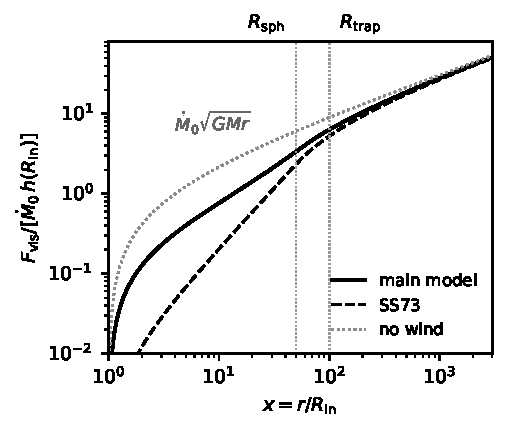
\includegraphics[width=\columnwidth]{torque_profile.pdf}
\caption{Viscous torque of a BH disc, Eq.~\eqref{eq:Fvis}, in units of $\Mdot_0 h(\rin)$, for the main accretion-rate profile (solid), the SS73 profile (dashed) and a disc without wind (dotted), $F_{\rm vis} = \Mdot_0[\sqrt{GMr} - \sqrt{GM\rin}] \to \Mdot_0\sqrt{GMr}$ at $r \gg \rin$.
Drawn for $\mdot_0 = 50$, $r_{\rm in,f} = 6$, $\Rsph = 6\mdot_0\rg$ ($\Rsph = 50\rin$), $f_{\rm in} = 0.3$, as in Fig.~\ref{fig:mdot_profiles} (Sect.~\ref{sec:radii:sph}).}
\label{fig:torque}
\end{figure}
% figure: this repository, figures/plot_torque_temperature.py (author's request 2026-11-21), computed from Eqs. (Fvis), (mdot_setin), (mdot_SS73)

\begin{figure}
\centering
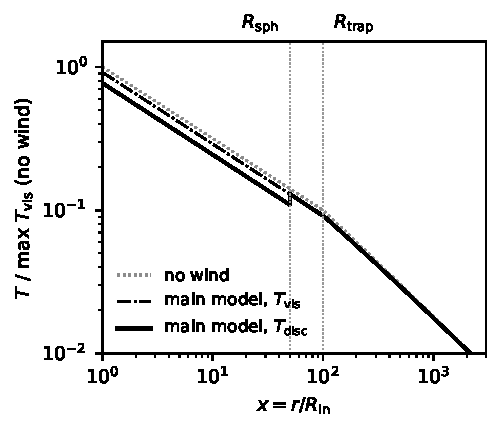
\includegraphics[width=\columnwidth]{temperature_profile.pdf}
\caption{Temperature of a BH disc: $\Tvis$ of Eq.~\eqref{eq:Teff} for the main accretion-rate profile (dash-dotted) and for a disc without wind (dotted), and the radiated temperature $T_{\rm disc}$ of Eq.~\eqref{eq:Tdisc} for the main profile with $\epsilon_{\rm w} = 0.5$ (solid), in units of the largest $\Tvis$ of the disc without wind.
Inside $\Rtrap = 12\mdot_0\rg$ (Eq.~\ref{eq:rtrap}) the temperature falls as $r^{-1/2}$, outside as $r^{-3/4}$; $T_{\rm disc}$ steps down inwards at $\Rsph$ by $(1 - \epsilon_{\rm w})^{1/4}$.
Parameters as in Fig.~\ref{fig:torque}.}
\label{fig:temperature}
\end{figure}
% figure: this repository, figures/plot_torque_temperature.py, computed from Eqs. (Fvis), (Qvis), (Teff), (Tdisc), (rtrap)

Figures~\ref{fig:streamlines_linear} and~\ref{fig:wind_geometry} (Sect.~\ref{sec:wind}) show the geometry of the wind at two fits.
The BH panel is the BH3a fit of NGC5408, made with the revised table of the transfer correction (190 runs): $M = 19.9\,M_\odot$, $\rin = 1.088\,r_{\rm isco} = 3.20\times10^6$~cm, $\log\mdot_0 = 2.153$, $\epsilon_{\rm w} = 0.387$, $\beta_{\rm w} = 2.68$, $\mdot_{\rm in}/\mdot_0 = 0.609$, $i = 50.3^\circ$ and $\omf = 0.7$.
Then $\Rsph = 1924\,\rin$, $\Rtrap = 1570\,\rin$ and $\rout = 2.57\times10^5\,\rin$; the wind photosphere covers $r = 94$--$6.6\times10^3\,\rin$ and rises to $z = 718\,\rin$, and the disc is seen directly inside and outside it.
The NS panel is the NS5r fit of NGC7793 with the dipole central emitter, made with the 117-run table ($\chi^2 = 0.94$ for 30 points): $M = 1.4\,M_\odot$, $\rmag = 6.48\times10^6$~cm, $\RNS = 0.154\,\rmag$, $\log\mdot_0 = 3.088$, $\epsilon_{\rm w} = 0.5$ and $\beta_{\rm w} = 1$ (fixed), $\mdot_{\rm in}/\mdot_0 = 0.0045$, $i = 17.3^\circ$, $\log\eta_{\rm magn} = 0$ and $\omf = 0.7$.
Then $\Rsph = 272\,\rmag$, $\Rtrap = 469\,\rmag$ and $\rout = 4.08\times10^8\,\rmag$; the wind photosphere covers $r = 1.29$--$2.8\times10^4\,\rmag$ and rises to $z = 4.4\times10^3\,\rmag$, and the disc is seen directly beyond about $3\times10^4\,\rmag$.
In both fits $\theta_{\rm c} = 45.6^\circ$ and $\theta_{\rm d} = 90^\circ$, so the outermost streamline runs along the disc.
% source: ULXspectra-mc docs/data/wind_geometry_params.md, commit 65f8bbf (calculation session 2026-11-21). BH: run mc28_0p3-10keV;
%         NS: run mc_0p3-10keV (NS5r chosen: NS7r, the best fit of NGC7793, has dip = 0; M51ULS NS6r has no wind, R_sph <= R_m);
%         the NS panel will be redrawn with the mc28 round's NGC7793 NS5r.

Figures~\ref{fig:streamline_speed} and~\ref{fig:streamline_speed_beta1} show the speed along the streamlines for the laws of Sect.~\ref{sec:wind:velocity}.

\begin{figure}
\centering
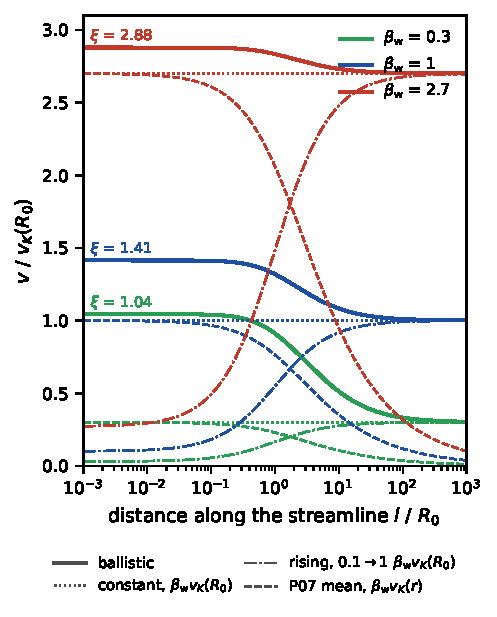
\includegraphics[width=\columnwidth]{streamline_speed.pdf}
\caption{Speed along the funnel-wall streamline ($\theta_0 = 45.6^\circ$) in units of $\vK(R_0)$, against the distance $l$ from the launch point in units of $R_0$, for $\beta_{\rm w} = 0.3$, 1 and 2.7 (colours) and the four laws (line styles): ballistic, Eq.~\eqref{eq:vballistic}; constant $\beta_{\rm w}\vK(R_0)$; rising, $v_0 + (v_\infty - v_0)\,l/(R_0 + l)$ with $v_0 = 0.1v_\infty$; and the P07 mean speed $\beta_{\rm w}\vK(r)$, held constant beyond $\Rsph$.
The ballistic speed starts at $\xi\vK(R_0)$, $\xi = \sqrt{\beta_{\rm w}^2 + 1} = 1.04$, 1.41 and 2.88, and falls to $\beta_{\rm w}\vK(R_0)$.
Made with \code{docs/scripts/plot\_streamline\_speed.py} (code commit eba4a0e).}
\label{fig:streamline_speed}
\end{figure}
% figure: ULXspectra-mc docs/figures/streamline_speed.pdf

\begin{figure}
\centering
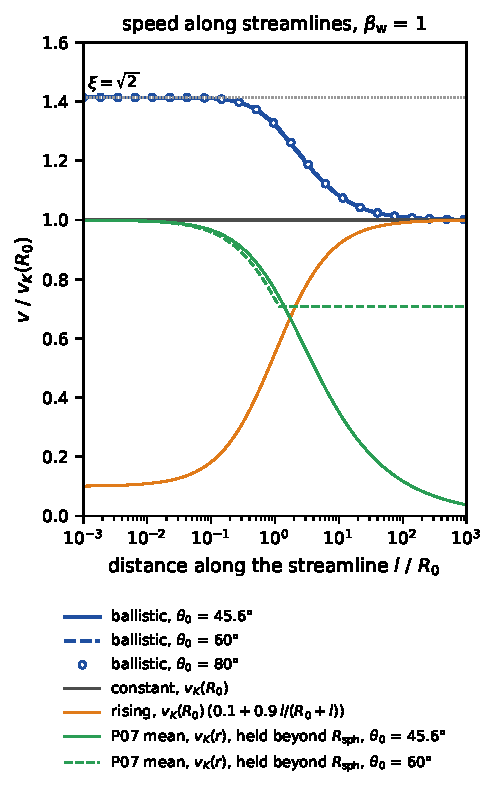
\includegraphics[width=\columnwidth]{streamline_speed_beta1.pdf}
\caption{As Fig.~\ref{fig:streamline_speed}, for $\beta_{\rm w} = 1$: the ballistic law at $\theta_0 = 45.6^\circ$ (solid), $60^\circ$ (dashed) and $80^\circ$ (open circles), which agree within 0.4\%, starting at $\sqrt2\,\vK(R_0)$ and falling to $\vK(R_0)$; and the comparison laws, constant, rising, and the P07 mean speed $\vK(r)$ held constant beyond $\Rsph = 1924\,\rin$, for $\theta_0 = 45.6^\circ$ and $60^\circ$.
Made with \code{docs/scripts/plot\_streamline\_speed.py} (code commit afb2f1f).}
\label{fig:streamline_speed_beta1}
\end{figure}
% figure: ULXspectra-mc docs/figures/streamline_speed_beta1.pdf
% AUTHOR: keep both speed figures, or only one?
% numbers: docs/wind_velocity_laws.md, commit 8920be0 (C model, 13 fits; max |dlog nuLnu| = 0.29 for BH4a at 0.003 keV)
% AUTHOR: keep this comparison here, or move it to the Discussion/Results after the refits?
% OUTLINE: figure vwind_laws.png (docs/scripts/compare_wind_velocity_laws.py, commit 35a22c0).
